
In Section~\ref{sec:development_of_a_parallel_k_d_tree_build_algorithm}, we introduced RQ~\ref{rq:parallel_build}, which questions the potential benefits if parallelizing the k-d tree build.   


\textbf{RQ~\ref{rq:parallel_build}.} \emph{It is possible to parallelize the k-d tree build algorithm, in such a way that it gives a significant speed improvement compared to the serial algorithm.}

The hard parallelization nature of the k-d tree was discussed and investigated, along the way some intermediate results was presented. 
we discussed the hard nature of parallelizing the k-d tree build. 


\begin{figure}[ht]
    \centering
    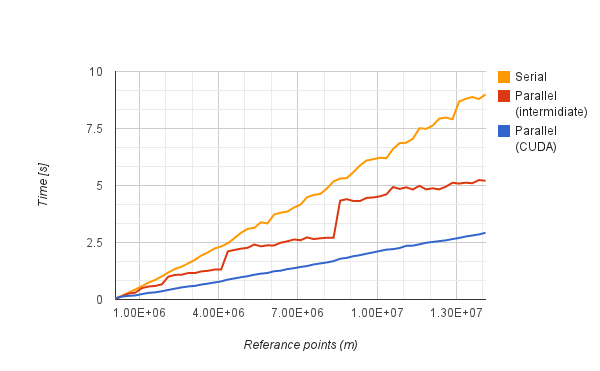
\includegraphics[width=120mm]{../gfx/final_tree_build.png}
    \caption{Comparison between serial and parallel k-d tree build performance.}
    \label{fig:final_tree_build}
\end{figure}

\begin{figure}[ht]
    \centering
    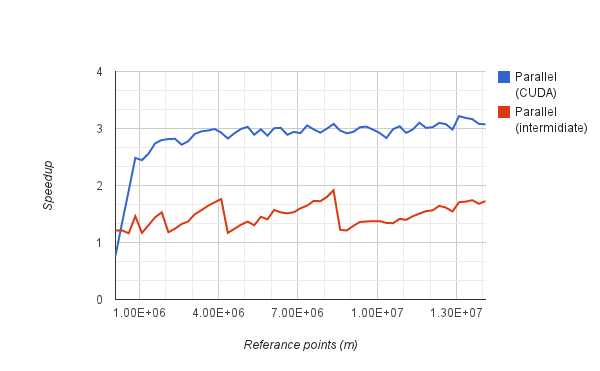
\includegraphics[width=120mm]{../gfx/final_tree_build_speedup.png}
    \caption{Parallel speedup for the k-d tree implementation for varying values of $m$.}
    \label{fig:final_tree_build_speedup}
\end{figure}



\textbf{RQ~\ref{rq:parallel_query}.} \emph{It is possible to parallelize the All-kNN query algorithm, in such a way that it gives a significant speed improvement compared to the serial algorithm.}


\begin{figure}[ht]
    \centering
    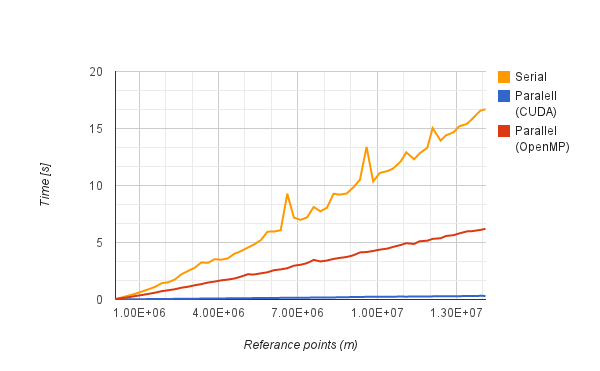
\includegraphics[width=120mm]{../gfx/final_kd_search.png}
    \caption{Comparison between serial and parallel All-kNN query performance.}
    \label{fig:final_kd_search}
\end{figure}

\begin{figure}[ht]
    \centering
    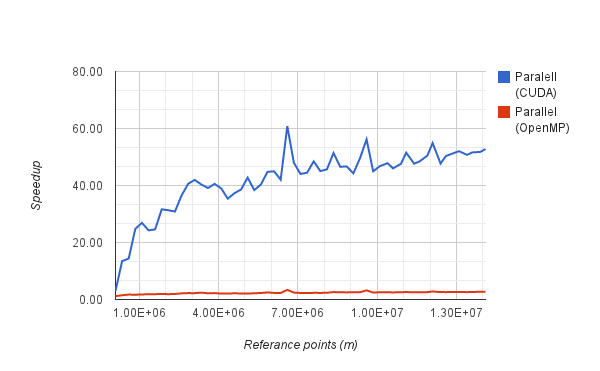
\includegraphics[width=120mm]{../gfx/final_kd_search_speedup.png}
    \caption{Parallel speedup comparison for the All-kNN query between the CUDA and OpenMP implementation.}
    \label{fig:final_kd_search_speedup}
\end{figure}



Graph of serial and parallel build, and query.

Some speedup calculation. Include Garcia as well, and point out that high speedup does not equal fast algorithm.
